\documentclass{standalone}
\usepackage{tikz}
\tikzset{%
  point/.style={circle,inner sep=1.25pt,minimum size=1.25pt,draw,fill=#1},
  point/.default=red
}
\definecolor{c0}{rgb}{0.2,0.4,0.67}
\definecolor{c1}{rgb}{0.67,0.4,0.12}
\definecolor{c2}{rgb}{0.53,0.6,0.13}
\definecolor{c3}{rgb}{0.53,0.53,0.4}
\begin{document}
\scalebox{2}{
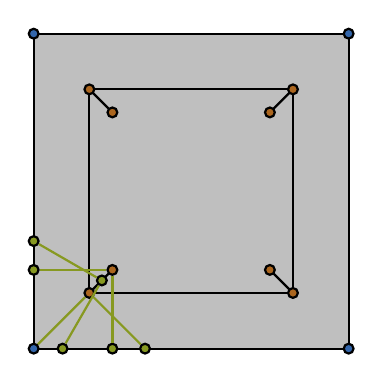
\begin{tikzpicture}[thick]
  \coordinate (p0) at (-2,-2);
  \coordinate (p1) at (2,-2);
  \coordinate (p2) at (2,2);
  \coordinate (p3) at (-2,2);
  \filldraw[fill=lightgray] (p0) -- (p1) -- (p2) -- (p3) -- cycle;%
  \node[point=c0] (m0) at (p0) {};
  \node[point=c0] at (p1) {};
  \node[point=c0] at (p2) {};
  \node[point=c0] at (p3) {};
  \coordinate (q0) at (-1.2929,-1.2929);
  \coordinate (q1) at (1.2929,-1.2929);
  \coordinate (q2) at (1.2929,1.2929);
  \coordinate (q3) at (-1.2929,1.2929);
  \coordinate (q4) at (-1,-1);
  \coordinate (q5) at (1,-1);
  \coordinate (q6) at (1,1);
  \coordinate (q7) at (-1,1);
  \draw (q0)--(q1);
  \draw (q1)--(q2);
  \draw (q2)--(q3);
  \draw (q3)--(q0);
  \draw (q0)--(q4);
  \draw (q1)--(q5);
  \draw (q2)--(q6);
  \draw (q3)--(q7);
  \node[point=c1] (n0) at (q0) {};
  \node[point=c1] (n1) at (q1) {};
  \node[point=c1] (n2) at (q2) {};
  \node[point=c1] (n3) at (q3) {};
  \node[point=c1] (n4) at (q4) {};
  \node[point=c1] (n5) at (q5) {};
  \node[point=c1] (n6) at (q6) {};
  \node[point=c1] (n7) at (q7) {};
  %%%
  \node[point=c2] (r0) at (-2,-1) {};
  \node[point=c2] (r1) at (-1,-2) {};
  \node[point=c2] (r2) at (-.5858,-2) {};
  \node[point=c2] (r3) at (-1.134,-1.134) {};
  \node[point=c2] (r4) at (-1.633,-2) {};
  \node[point=c2] (r5) at (-2,-.634) {};
  \draw[c2] (r0)--(n4)--(r1);
  \draw[c2] (m0)--(n0)--(r2);
  \draw[c2] (r4)--(r3)--(r5);
\end{tikzpicture}
}
\end{document}
